%% example.tex
%% Jeremy Singer
%% 16 Oct 12

\documentclass{mpaper}

\usepackage{lipsum}
\usepackage{graphicx}
\usepackage{float}
\usepackage{algorithm}
\usepackage{algpseudocode}
\usepackage{caption}
\usepackage{subcaption}
\graphicspath{{images/}}
% \usepackage{mathtools, cuted}

\begin{document}

\title{Spatial Smoothing in Mass Spectrometry Imaging}
\author{Arijus Pleska}
\matricnum{2019828P}

\maketitle

% ___________________________________________________________________________
\begin{abstract}
Lorem ipsum dolor sit amet, consectetuer adipiscing elit. Ut purus elit, vestibulum ut, placerat ac, adipiscing vitae, felis. Curabitur dictum gravida mauris. Nam arcu libero, nonummy eget, consectetuer id, vulputate a, magna. Donec vehicula augue eu neque. Pellentesque habitant morbi tris- tique senectus et netus et malesuada fames ac turpis egestas. Mauris ut leo. Cras viverra metus rhoncus sem. Nulla et lectus vestibulum urna fringilla ultrices. Phasellus eu tellus sit amet tortor gravida placerat
\end{abstract}

% ___________________________________________________________________________
\section{Introduction}

% Purpose:
% - A spatial smoothing application in visual data using unsupervised ML
% - Focus: Metabolomics and topic modelling
\par In this research paper, we assess an application of spatial smoothing in visual data; that is, we induce continuity among data elements. The spatial smoothing application is particularly targeted to be applied for unsupervised pattern recognition. To be more specific, our focus is to model a biomedical application in the field of metabolomics. Furthermore, we limit the scope of the applied unsupervised machine learning techniques to the branch of topic modelling.  

% Basis:
% - Visual data: MSI application in metabolomics
% - MSI data structure
\par The characteristics of our utilised metabolomics data are expressed in the form of mass spectrometry imaging (MSI). Effectively, we use MSI to visualise the metabolomics data in the form of spatial distribution. Speaking of the metabolomics data, it contains information about ionised metabolites. Note that metabolites are molecules produced by the chemical process of metabolism; whereas by ionisation, we refer to the method used to sample metabolites. In other words, MSI data is a visualisation of ion (sampled metabolite) distributions: the complete dataset is the whole image; the image's pixel is a particular sampling region; and each region contains intensities of ions with unique mass-over-charge $m/z$ values. 

% Basis:
% - Unsupervised machine learning: Topic modelling
% - topic modelling w.r.t. MSI
\par Speaking of our machine learning application, topic modelling is a technique used to infer unlabelled topic distributions based on data's underlying semantic structure. With respect to MSI data, we can model the topic distributions over an image and its every pixel; furthermore, topic modelling can express the types of ions corresponding to particular topics. Since a topic model is a statistical approach to perceive real metabolomics data, the utilised topic models are tuned to reflect the metabolomics environment as good as possible. Relating to our research targets, spatial smoothing is one of such environment settings.

% Research Problem:
% - Noisiness
% -- Fragmentation
% -- Retention time
% - Loss of information
% -- Overlapping topics
\par The basis of the project's research problems comes from the limitations of current metabolite sampling techniques. The main limitation is the loss of information caused by the metabolite ionisation. As a consequence, the MSI data is noisy. To expand on the noisiness, it is caused by metabolite fragmentation and the limitation to tune different metabolite retention times. By metabolite fragmentation, we refer to a metabolite split; the split would cause the captured ions to possess unexpected values. Speaking of the retention time, the intensity value of each ion types varies with respect to time; therefore, since each ion is captured at a different state of its retention, each ion type would possess some variance with respect to its intensity. Finally, note that the loss of information might be also caused by overlapping ion topics. Since different ion topics can contain same ion types, the topic possessing a lower ion intensity value would be overwhelmed and, thus, not reflected in the MSI data.
% Contributions:
% - A specific and extensive assessment of the SS application
% - A tuned topic model and well-organised experiment settings
\par In this paper, we contribute to the research in MSI by carrying an extensive assessment of the spatial smoothing application. The assessment is carried in both quantitative and qualitative manners: we assess the performance on a number of diverse datasets; also, our experiments are designed to reflect the nature of the MSI data reflecting computational metabolomics. Furthermore, we provide a Python implementation of a tuned topic model; also, we establish maintainable experiment settings. By the tuned topic model, we mean that the model's implementation is particularly designed to meet the characteristics of the MSI data. Speaking of the experiment settings, note that we are carrying the experiments using Jupyter notebooks. Effectively, the use of the notebooks creates a portable and well-documented environment to initialise the experiment settings and execute the topic modelling. As a result, external parties could run the released notebooks and reproduce the experiment results in a swift manner.

% The paper's organisation
\par The paper is organised in the following order: in Section 2, we discuss the background of the research project; in Section 3, we provide a formal definition of the assessed research problems; in Section 4, we review the results of the relevant research; in Section 5, we establish the rationale of the applied methodology; in Section 6, we introduce the experiments results; finally, in Section 7, we conclude the findings. 

% ___________________________________________________________________________
\section{Background}

% Intro
% - Preliminaries: Introduce the rationale of LDA
% - Terminology: Define the applied topic modelling terminology
% - MSI Data characteristics: Introduce the qualities of the data
\par The background section covers the basis of the concepts used throughout the paper. At the start, we provide a high-level overview of the general topic modelling concepts. Then, we define the terminology used throughout the paper. Finally, we introduce the characteristic qualities of the MSI data.  

\subsection{Topic Modelling Preliminaries}

% LDA Intro:
% - Hierarchical structure
% - Generative model
% - Bayesian methods
% - Assumptions
\par The research project targets a specific branch of topic models. The branch consists of Latent Dirichlet Allocation (LDA) derivatives. Note that the initial LDA model was introduced by Blei et al. \cite{blei2003latent}. One of the model's key characteristics is the three-level hierarchical treatment of the data. In the context of the utilised MSI data, the hierarchical structure can be perceived as follows: in the highest level, we have an MSI image; in the middle level, we have a pixel of an MSI image; and in the lowest level, we have the intensities of particular ions in a pixel.

% Generatitive model:
% - Generative process
\par Another model's key characteristic is the generative treatment of the data. By the generative model, we mean that the latent data instances are treated as a result of a mixture of underlying parameters drawn from probability distributions. In other words, the generative data treatment induces randomness in the end products of the data; however, note that the source of the data -- the lowest level parameters of the probability distributions -- remain the same. The key aspect of the generative model is the degree of freedom in the connections of random variables; this notion allows modelling more realistic, thus, more complex data relations. Ultimately, the rationale of the generative model is based on recovering the underlying semantic structure. Effectively, in order to recover the generative process of the data, we delve into the applications of Bayesian methods.

% Bayesian methods
% - Inference: sampling
% - Connection to LDA
\par By applying Bayes' rule, we can express the underlying semantic structure can be expressed in the form of posterior probability distributions. However, note that we can not analytically compute such posterior expressions. Instead, we can estimate the the posterior distributions using optimisation or direct sampling. In this project, we particularly focus on the underlying semantic structure's inference using direct sampling. Speaking of the sampling-based inference method applications to LDA-like models, the ground-work has been established by Griffiths and Steyvers \cite{griffiths2004finding}. The authors have utilised a collapsed Gibbs sampling -- a Markov chain Monte Carlo (MCMC) algorithm -- in order integrate the uncertainty out and sample only the parameters of interest. More specific details about the rationale of the collapsed Gibbs sampling application will be provided in Section 4. 

% Assumptions
% - Exchengeability (BoW)
% - Discrete data
\par Relating to the initial LDA model, the authors have set the following assumptions for the utilised data: exchangeability among the inner components of the lower and middle data hierarchy levels; and discrete treatment of the lower-level data. By exchangeability, it is meant that the components follow the bag-of-words principle; that is, the order of the data has no correlation with the underlying semantic structure. Speaking of the discrete data treatment, it is assumed that the lower-level components have no spatial connection. With respect to our project, both assumption types -- exchangeability and discreteness -- do not correspond to the characteristics of the MSI data. Therefore, we will establish a methodology to relax the latter assumptions.

\subsection{Topic Modelling Terminology}

% Terminology intro:
% - Introduce the three-level hierarchical structure
\par In this subsection, we introduce the topic modelling terminology. In order to put the MSI data in the topic modelling context, the components of  LDA's three-level hierarchical structure are defined as follows: \textit{the corpus} is the whole image of a sample; \textit{the document} is an MSI image's pixel; and \textit{the word} is an interval of mass-over-charge values corresponding to a particular ion. Starting from now on, we will use the latter topic modelling concepts to introduce the LDA model's architecture and notation.

% LDA design
% - Graphical model
\par Since LDA-like models are also graphical models, the dependence of random variables can be illustrated using graphs. In order to familiarise with the architecture and the variables of LDA-like models, we provide Figure \ref{fig:arch_LDA-init} illustrating the initial LDA model in the plate notation.
\begin{figure}[h]
  \centering
  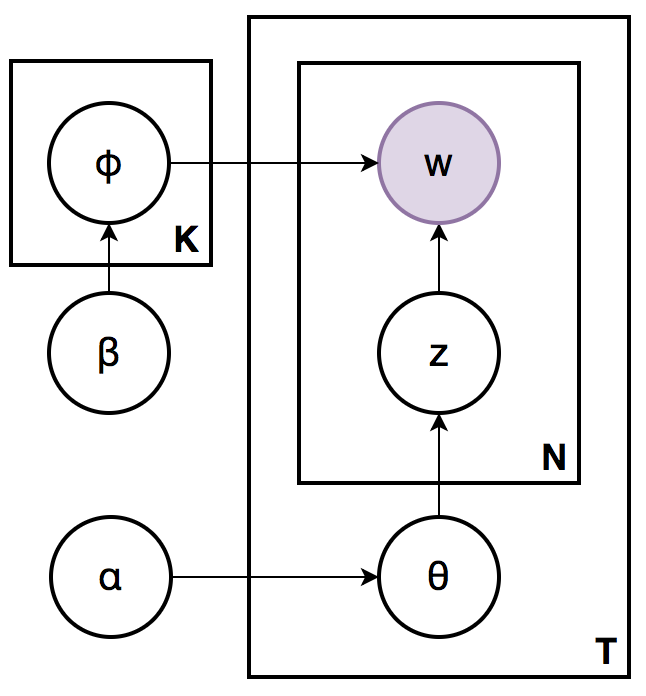
\includegraphics[width=0.25\textwidth]{LDA-initial.png}
  \caption{The initial LDA model's architecture.}
  \label{fig:arch_LDA-init}
\end{figure}
The circles indicate the model's variables: the coloured circle corresponds to the observable variable, whereas the uncoloured circles corresponds to the hidden variables. Effectively, the hidden variables define the model's underlying structure. Speaking of the plates, the plate denoted by $K$ corresponds to the number of topics; the plate denoted by $T$ corresponds to the number of documents and the plate denoted by $N$ corresponds to the number of words. Effectively, the letters in the bottom right corners indicate the total number of variables. Therefore, a corpus has $T$ number of documents, and each document has $N$ number of words.

% Terminology
% - Parameter meaning
% - Listing
\par Before providing a listing with the definitions of the LDA variables, we will briefly introduce the purpose of the variables. The variables denoted by $\theta$ and $\phi$ correspond to the underlying probability distributions (e.g., in the case of the initial LDA model, we use Dirichlet distributions). It follows that the variables denoted by $\alpha$ and $\beta$ act as the parameters of the latter probability distributions; note that in the context of machine learning, such auxiliary parameters are called hyper-parameters. Effectively, \textit{a hyper-parameter} allows to tune a machine learning model for a particular dataset application. As a side reference, note that by \textit{a vocabulary} we refer to a collection of terms reflecting a fixed range of the words. At this point, we provide the following list containing the definitions of the initial LDA model's variables: 
\begin{itemize}
	\item $K$ is the number of topics;
	\item $T$ is the number of documents;
	\item $N$ is the number of words per document;
	\item $V$ is the size of a vocabulary;
	\item $w$ is a word;
	\item $z$ is a word's topic assignment;
	\item $\theta_t$ is the topic distribution over document $t$;
	\item $\phi_k$ is the vocabulary term distribution over topic $k$;
	\item $\alpha$ is the hyper-parameter for the topic distributions;
	\item $\beta$ is the hyper-parameter for the vocabulary term distributions.
\end{itemize}

\subsection{MSI Data Characteristics}

% MSI dataset intro:
% - Introduce the raw data format
% - Describe the data pre-processing requirements
\par In this subsection, we will introduce the qualities of the raw MSI data. Furthermore, we will set the requirements for the raw data's pre-processing; note that the pre-processing serves as an auxiliary method making the raw MSI data compatible for a scalable topic modelling application. As a side note, the basis of our applied MSI data characteristics is established from the mzML data format. Conveniently, we have parsed the mzML data format using the \texttt{pymzml} Python library. 

% Raw data format
% - Data meaning
% - Explain the raw data by looking into it
\par Essentially, raw MSI data contain mass spectra of a sample -- the sample's every pixel is expressed in the form of a mass spectrum. By a mass spectrum, we refer to a map of from a mass-over-charge value to an intensity value. Ultimately, we can establish a continuous notion of the MSI data by ordering the mass-over-charge values. Note that since the sampling equipment can detect the mass-over-charge values in the millidalton (mDa) precision, the MSI data is sparse (i.e., a large portion of mass-over-charge values are mapped to the zero intensity).

% Data pre-processing requirements
% - Vocabulary generation
% - Intensity normalisation
% - Dismissing inferior information
\par In the context of topic modelling, the raw MSI data possess a large vocabulary (above $5000$ terms). Note that we consider every mass-to-charge value as a word; whereas every intensity value is perceived as a word occurrence count. Further, since the intensity values could spike up above $1000$, the time complexity of the latent topic inference would require pro-longed runs. To overcome the introduced scalability issues, we have carried data pre-processing -- the applied techniques are discussed in the upcoming methodology section.

% ___________________________________________________________________________
\section{Statement of Problem}

% Hypothesis
% - A topic is continuous throughout nearby regions
\par To start with, we set the hypothesis of this research project to \textit{`The noisiness of MSI pixels can be reduced by applying a topic model tuned for spatial smoothing'.} By spatial smoothing, it is meant that the topic model would have an auto-regressive treatment among the pixels. As an example, we assume that adjacent pixels would have similar latent topic distributions. This assumption corresponds to the nature of our datasets -- a metabolite construction (i.e., a topic) is continuous throughout nearby regions (i.e., sets of adjacent pixels).

% Contributions
% - Naive AR model application
% - Motivating for the state-of-the-art AR model application
\par The impact of proving the hypothesis would bring the following contributions:
\begin{itemize}
	\item Improving the detection of overlapping topics;
	\item Reducing the noisiness of MSI data;
	\item Motivating the further research in applying spatial \\smoothing to MSI data.
\end{itemize} 
To expand on the overlapping topic detection, the issue arises when two underlying topics are made of similar vocabulary terms: instead of a separate representation, the topics are merged. We intend to identify the flow of distinct topics by the application of spatial smoothing; as a consequence, the spatial smoothing would also impact the data noisiness reduction. Ultimately, if a naive spatial smoothing application displayed a performance improvement, the contribution would set a basis to utilise state-of-the-art auto-regression techniques on MSI data.

% Approach
% - Clearly define the experiment settings
% - Tune the models by studying synthetic datasets.
\par To my knowledge, the impact of the spatial smoothing application to the MSI domain has not yet been thoroughly studied. For the latter reason, this research project will serve as an exploratory assessment on the spatial smoothing application: we will introduce the rationale behind the applied methodology; also, we will clearly define the range of the experiment settings. To give a brief intuition about the methodology, the study will assess the domain-specific parameter tuning and its impact on a diverse range of synthetic datasets.

% ___________________________________________________________________________
\section{Relevant Research}

% Intro (separate into three)
% - MSI DATA:
% -- alonso2015analytical
% -- Review the metabolomics feature pre-processing
% -- Review the metabolomics alternative approaches
% - Review the implementation approaches
% -- blei2012probabilistic
% -- Gibbs sampling
% -- DTM
\par In this section, we will review the groundwork on the following aspects: the pre-processing of MSI data; the rationale of the utilised topic models; and novel approaches exploiting the characteristics of MSI data. Note that the covered groundwork is selected to reflect the rationale of the utilised techniques. In order to establish the basis of the state-of-the-art computational metabolomics methodology, we have consulted the survey carried by Alonso et al. \cite{alonso2015analytical}; speaking of the key probabilistic topic modelling branches, we have consulted the survey carried by Blei \cite{blei2012probabilistic}. 

\subsection{MSI Data Pre-processing}

% Metabolomics: feature pre-processing
% - Normalisation:
% -- kohl2012state
% -- bolstad2003comparison

\par In order to establish a scalable topic inference, we review the following MSI data pre-processing techniques: data normalisation; feature binning; and noise reduction. To start with, data normalisation serves as a method establishing an integrable data structure. Bolstat et al. \cite{bolstad2003comparison} have proposed a data normalisation method called linear baseline scaling. Note that the method is particularly targeted at sparse datasets. Effectively, the method is applied on numerical features by executing the following work-flow: we find the largest numerical feature of all data instances; then, we calculate the scaling factors by aligning the largest values to a pre-set upper threshold; finally, we align the remaining numerical features based on the established scaling factors. Relating linear baseline scaling to applications on MSI data, Kohl et al. \cite{kohl2012state} have shown that the method's application does not produce a significant loss of information for a well-performing MSI data inference. 

% - Binning
% -- Evenly spaced 
% -- craig2006scaling
% -- Spectral peaks
% -- de2008nmr
\par Speaking of feature binning, the technique is used to merge the instances of a feature space; as a result, feature binning reduces the data dimensionality. Note that by the MSI data feature space, we refer to distinct $m/z$ values. Since raw MSI data is sparse, a successful application of feature binning is based on identifying appropriate $m/z$ boundaries reflecting unique metabolite types. To introduce some examples, the research carried by Craig et al. \cite{craig2006scaling} have utilised an equally spaced feature binning. Even though the authors have succeeded to reduce the data dimensionality, they have encountered a loss of information by splitting the metabolite topics into arbitrary regions. As an alternative approach, De et al. \cite{de2008nmr} have performed a feature binning based on the spectral peak identification. Effectively, the technique induces a dynamic notion of bin boundaries which is based on the identified intensity peak regions. As a result, the merged $m/z$ values serve as a better representation of metabolite terms.

% - Denoising (removing small intensities)
% -- smith2014proteomics
\par The last reviewed MSI data pre-processing techniques addresses the MSI data noisiness. Even though the MSI data noise reduction is an open research problem going well beyond data pre-processing, Smith et al. \cite{smith2014proteomics} have shown that the application of a general data pre-processing routine displays performance improvements. For example, the authors have induced a lower intensity bound. Effectively, the intensity values below the intensity threshold would be treated as insignificant and/or as a product of data capturing device imperfections. By applying this procedure, the authors have successfully reduced the data dimensionality and, thus, increased the data scalability.

\subsection{Prospective Topic Models}

% Intro
% - Inference
% - Derivatives
% - Gibbs sampling
% -- griffiths2004finding
\par In this subsection, we review the key characteristics of the prospective topic modelling inference techniques and model variations. Speaking of the inference techniques, we have employed the rationale of a sampling-based LDA model. Griffiths and Steyvers \cite{griffiths2004finding} have displayed a successful application of the collapsed Gibbs sampler for the topic inference of both textual and visual data. To expand on the collapsed sampling, the technique allows skipping the estimation of $\theta$ and $\phi$ values; instead, the inference is based on the notion of the assignment counts. In order to estimate a topic assignment's probability, the authors suggest using the following expression:
\begin{equation*}
p(z_i = k | z_{-i}, w) \propto \dfrac{n_{-i, k}^{(w_i)} + \beta}{n_{-i, k}^{(\cdot)} + V\beta}\cdot \dfrac{n_{-i, k}^{(t_i)} + \alpha}{n_{-i, \cdot}^{(t_i)} + K\alpha}.
\end{equation*}
note that $i$ refers to the current iteration ($-i$ refers to the previous iteration); $k$ refers to a particular topic; and $n$ refers to the count of the instances indicated by the term's superscript. If required, $\theta$ and $\phi$ can be sampled from the following distributions:
\begin{align*}
\phi_{k,w} & \sim \mbox{Dirichlet}\bigg(\dfrac{n_{k}^{(w)} + \beta}{n_{k}^{(\cdot)} + W\beta}\bigg),\\
\theta_{t,k} & \sim \mbox{Dirichlet}\bigg(\dfrac{n_{k}^{(t)} + \alpha}{n^{(t)} + K\alpha}\bigg).
\end{align*}
Essentially, more accurate representations of $\theta$ and $\phi$ are obtained by running the Gibbs sampler until a sufficient convergence: we preserve the $\theta$ and $\phi$ values of each iteration; when the sampling is finished, the average of the preserved values is an accurate approximation of the underlying $\theta$ and $\phi$ values.

% Topic modelling:
% - DTM
% -- blei2006dynamic
% - SeqLDA
% -- du2012sequential
\par In order to relax the topic modelling assumptions of the initial LDA model, we review the model's derivatives. One of the assumptions -- word exchangeability -- is addressed by Blei and Lafferty \cite{blei2006dynamic}. 
The authors have proposed dynamic topic model (DTM) inducing the notion of change in topic and vocabulary distributions; the model's architecture is illustrated in Figure \ref{fig:arch_dtm}.
\begin{figure}[h]
  \centering
  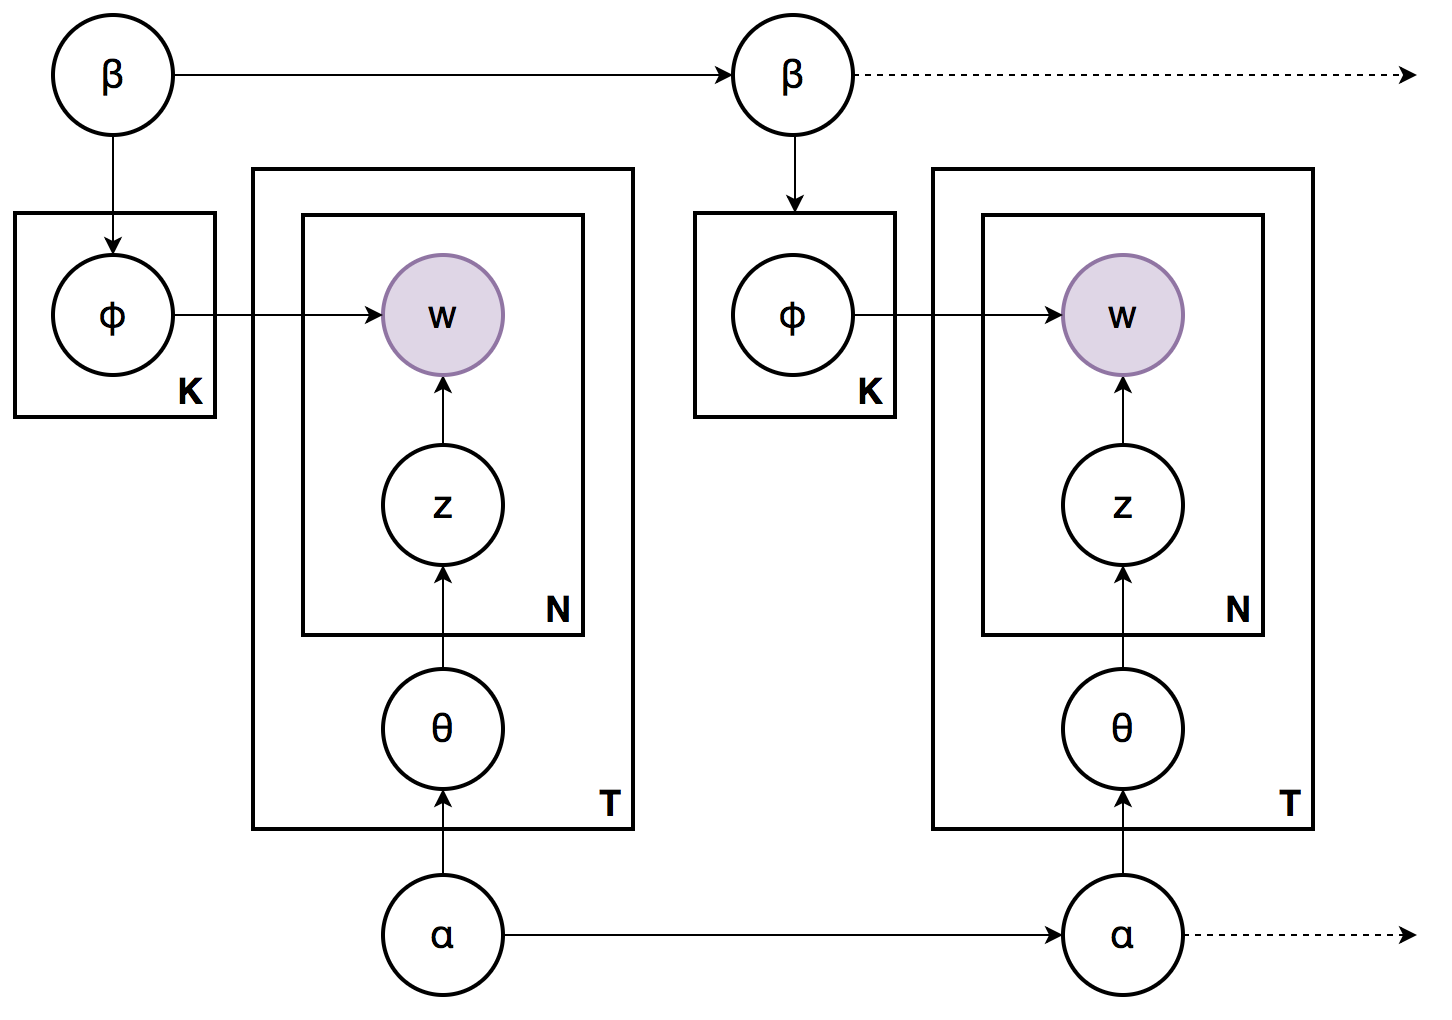
\includegraphics[width=0.4\textwidth]{dtm-architecture.png}
  \caption{The DTM architecture.}
  \label{fig:arch_dtm}
\end{figure}
Ultimately, the documents of a corpus are assigned to segments with unique $\theta$ and $\phi$ values. Note that the changes in $\theta$ and $\phi$ values are impacted by their hyper-parameter updates. Since in DTM's paper the authors use variational inference, we provide a reference into an alternative dynamic topic modelling variation -- sequential LDA -- proposed by Du et al. \cite{du2012sequential}. Note that in the sequential LDA's paper, the authors display a rigorous application of the collapsed Gibbs sampler. 

\subsection{Prospective Characteristics of MSI Data}
% Metabolomics: spatial smoothing
% - TM application
% -- van2016topic
\par At this point, we look into the prospective topic modelling applications exploiting the characteristics of MSI data and employing spatial smoothing. To start with, Hooft et al. \cite{van2016topic} have utilised an LDA-like model to infer metabolite substructures from MSI data. The authors have established a novel approach utilising a favourable LDA's property -- the option to assign a unique vocabulary term to multiple topics. Effectively, this approach allows identifying metabolite substructures which are made of overlapping elements. 

% - Spatial Chaos
% -- palmer2016fdr
\par Speaking of the spatial smoothing application, to my knowledge, the idea has not yet been widely spread among the computational metabolomics community. Nevertheless, a recent study by Palmer et al. \cite{palmer2016fdr} have attempted to quantify spatial chaos among the partitions of MSI data. The authors have reported that the established notion of spatial chaos have improved the speed and accuracy of continuous metabolite pattern identification. 


% ___________________________________________________________________________
\section{Methodology}

% Intro
\par In this section, we cover the rationale of a topic model tuned for a spatial smoothing application. To start with, we provide details on how to establish the auto-regressive notion among MSI data. Then, we show how to apply the auto-regression to a topic inference based on the collapsed Gibbs sampling. Further, we provide a list of the applied data pre-processing techniques for MSI data. Finally, by considering the data format induced by the pre-preprocessing, we introduce the generative MSI data process. Effectively, we apply the generative process to generate synthetic data for our experiments.

\subsection{Spatial Smoothing}

% Introduce AR
% - Define the first two variances
% - Point out that we are using the terms corresponding to the MSI data
\par We establish the spatial smoothing among MSI data by inducing the auto-regressiveness among the pixels (documents). Before going into details, note that we cover the established methods using the previously introduced topic modelling notation. To start with, recall that by auto-regressiveness we refer to the smooth topic development among the nearby instances of an MSI corpus. In our settings, the auto-regressiveness is established by assuming that the joint probability distribution of the $\alpha$ priors is given by the following expression:
\begin{align*}
&p(\alpha_1,\ldots,\alpha_T) =p(\alpha_1)\prod_{t=2}^{T}{p(\alpha_t|\alpha_{t-1})}, \quad \mbox{where}\\
&p(\alpha_0) =\mathcal{N} (\alpha_0; 0, \sigma_0^2I), \quad \mbox{and}\\
&p(\alpha_t) =\mathcal{N} (\alpha_t; \alpha_{t-1}, \sigma^2I), \quad t>1.
\end{align*}
To introduce the previous expression, note that index $t$ refers to a particular pixel (a document). This means that every pixel of an MSI corpus has a unique underlying topic distribution induced by a unique $\alpha$. Further, variances $\sigma_0^2$ and $\sigma^2$ correspond to the initialisation variance and the smoothness variance, respectively. Effectively, $\sigma_0^2$ is used to create larger gaps among different topics, whereas $\sigma^2$ preserves the smoothness. Therefore, we set $\sigma_0^2$ to possess a higher value compared to $\sigma^2$.

% Introduce the MH algorithm
\par The previously introduced $\alpha$ priors serve as the initial point in estimating the true $\alpha$ values. To estimate the true $\alpha$ values, we utilise the Metropolis--Hastings (MH) algorithm. The work-flow of the MH algorithm is started by drawing the proposed state
\begin{align*}
&x' \sim q(x,\delta^2I).
\end{align*}
Note that $x$ denotes the current state, $q$ denotes the proposal distribution, and $\delta^2$ denotes the proposal variance. Note that if $\delta^2$ is large, the proposal state converges to the true posterior in larger yet random increments; alternatively, if $\delta^2$ is small, the convergence is performed in small yet uniform increments. Note that the settings for optimal convergence are unique for diverse datasets; as an example, we can find the optimal values using cross validation. Going back to the work-flow, for the second step, we consider the acceptance distributions (these are denoted by $A$) and derive the formula for the acceptance rate:
\begin{align*}
  \dfrac{A(x'|x)}{A(x|x')} = \dfrac{p(x'|x)}{p(x|x')}\cdot \dfrac{q(x'|x)}{q(x|x')} = \dfrac{p(x',x)}{p(x)}\cdot \dfrac{p(x')}{p(x,x')} = \dfrac{p(x')}{p(x)}.
\end{align*}
Note that the proposal distributions cancel out as
\begin{align*}
q = \mathcal{N} \quad \Longrightarrow \quad q(x'|x) = q(x|x').
\end{align*}
For the MH algorithm's final step, we make sure that the acceptance rate does not overflow the probability boundaries; that is, we obtain the acceptance rate denoted by $r$ using the following procedure:
\begin{align*}
  r = \min{\bigg(1, \dfrac{p(x')}{p(x)}\bigg)}.
\end{align*}

% Apply the MH algorithm to the MSI data
% TODO: Softmax
\par At this point, we apply the rationale of the introduced MH algorithm to the topic modelling context. Since we utilise the MH algorithm to update a single value at a time (i.e., we update $\alpha_{t,k}$), we make use of the following notation:
\begin{align*}
  \alpha^{-tk} = \alpha \setminus \alpha_{t,k}.
\end{align*} 
Having the previous notation in mind, the MH algorithm's application to update $\alpha$ is given as follows:
\begin{align*}
  &\dfrac{p(z,\alpha^{-tk},\alpha_{t, k}'|X)}{p(z,\alpha|X)} = \ldots\\
  &\ldots = \dfrac{p(X|z,\alpha^{-tk},\alpha_{t, k}')}{p(X|z,\alpha)}\cdot \dfrac{p(z|\alpha^{-tk},\alpha_{t, k}')}{p(z|\alpha)}\cdot \dfrac{p(\alpha^{-tk},\alpha_{t, k}')}{p(\alpha)}\\
  &\dots = \dfrac{\prod_{k=1}^K\pi(\alpha_{t,k}')^{z_{t,k}}\cdot p(\alpha_t'|\alpha_{t-1})\cdot p(\alpha_{t+1}|\alpha_t')}{\prod_{k=1}^K\pi(\alpha_{t,k})^{z_{t,k}}\cdot p(\alpha_t|\alpha_{t-1})\cdot p(\alpha_{t+1}|\alpha_t)};\quad t \not\in \{1,T\}.
\end{align*}
For completeness, the expressions at the boundaries take the following form:
\begin{align*}
t=1 \quad \Longrightarrow \quad &\dfrac{p(\alpha^{-1k},\alpha_{1, k}')}{p(\alpha)} = \dfrac{p(\alpha_{1}')\cdot p(\alpha_{2}|\alpha_{1}')}{p(\alpha_{1})\cdot p(\alpha_{2}|\alpha_{1})},\\
t=T \quad \Longrightarrow \quad &\dfrac{p(\alpha^{-Tk},\alpha_{T, k}')}{p(\alpha)} = \dfrac{p(\alpha_{T}'|\alpha_{T-1})}{p(\alpha_{T}|\alpha_{T-1})}.\\
\end{align*}
Also, note that by $\pi$ we denote the softmax function which is expressed as follows:
\begin{align*}
  \pi(\alpha_{t,k}) = \dfrac{\exp(\alpha_{t,k})}{\sum_{k'=1}^K \exp(\alpha_{t,k'})}
\end{align*} 

\subsection{Auto-regressive Dynamic Topic Model}

% Intro
% - Model modifications
\par Our auto-regressive topic model is based on the rationale of the reviewed dynamic topic model. However, based on the MSI data characteristics and the application of spatial smoothing, the auto-regressive model possesses the following aspects:
\begin{itemize}
	\item The static treatment of the $\beta$ hyper-parameter;
	\item The Gibbs sampler utilising spatial smoothing;
	\item The application of logarithmic space to perform calculations.
\end{itemize}
In the following paragraphs, we will introduce each of the previous listings.

\par Even though we utilise the rationale of DTM in order to establish the dynamic notion in the topic development, we preserve a static $\beta$ hyper-parameter. This assumption comes from the characteristics of the metabolomics-based MSI data: we expect the metabolite patterns (i.e., a topic's vocabulary) remain constant. Therefore, in our model, we utilise the architecture illustrated in Figure \ref{fig:arch_ar} below.
\begin{figure}[H]
  \centering
  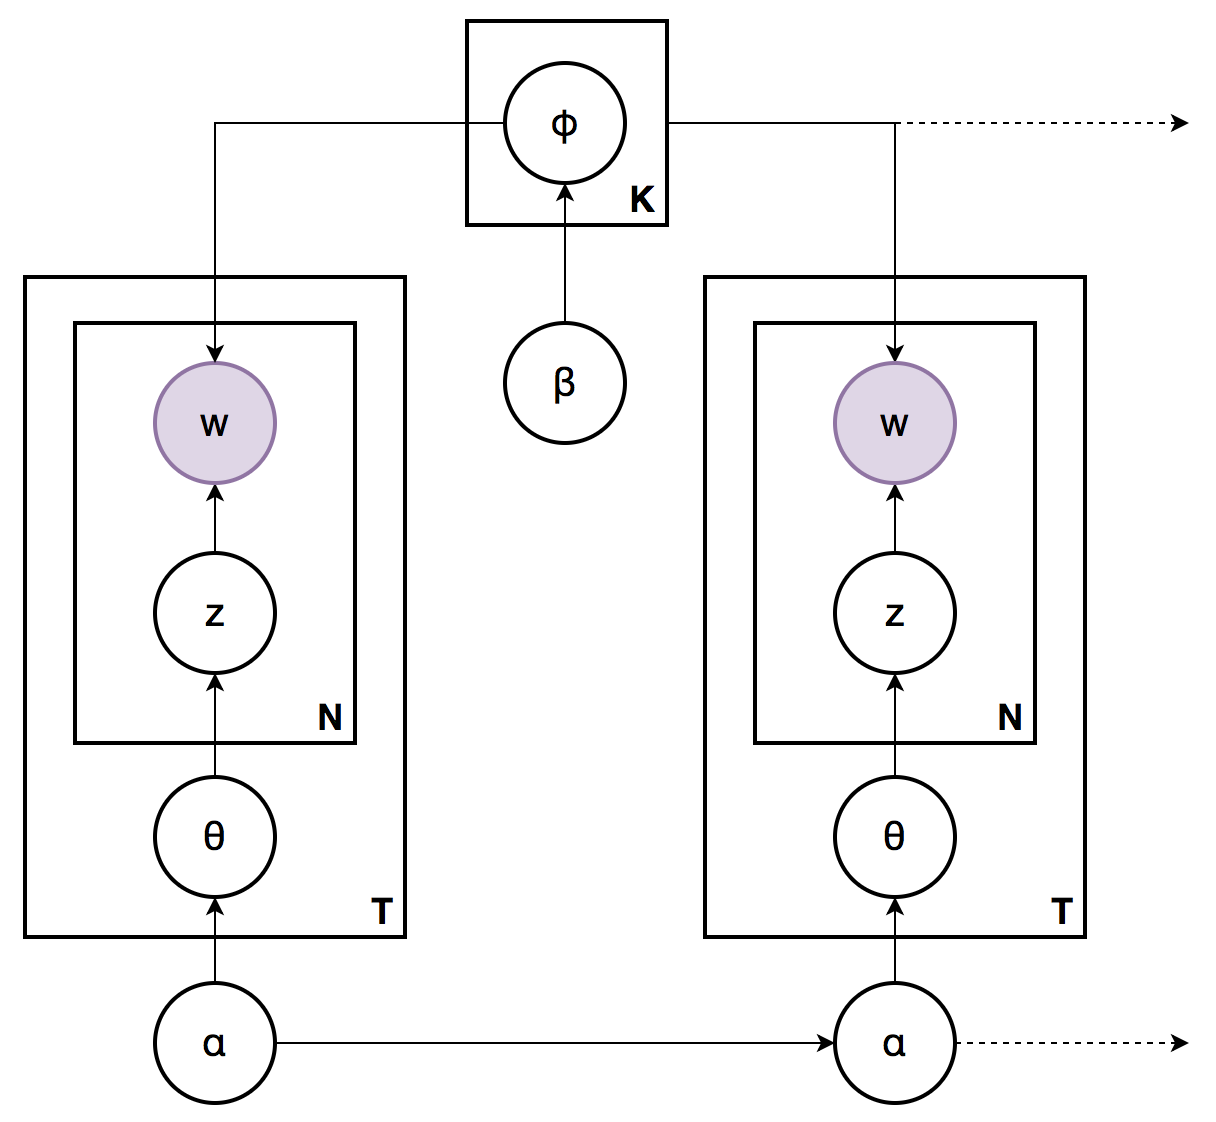
\includegraphics[width=0.4\textwidth]{ar-architecture.png}
  \caption{The auto-regressive topic model architecture.}
  \label{fig:arch_ar}
\end{figure}

% Gibbs Sampler changes
\par Speaking of the Gibbs sampler's enhancement, the updated topic assignment formula takes the following form:
\begin{equation*}
p(z_i = k | z_{-i}, w, t) \propto \dfrac{n_{-i, k}^{(w_i)} + \beta}{n_{-i, k}^{(\cdot)} + V\beta}\cdot \pi(\alpha_{t,k}).
\end{equation*}
As a consequence, the sampling of $\theta$ also changes; now, we draw the topic distributions by carrying the following procedure:
\begin{align*}
\theta_{t,k} & \sim \mbox{Dirichlet}\big(\pi(\alpha_{t,k})\big).
\end{align*}

% Calculations in the log space
\par Finally, we address the computational stability by performing calculations in logarithmic space. Effectively, the application of logarithmic space mitigates the susceptibility to numerical underflow. Note that numerical underflow is especially relevant in the context of probabilistic models: calculations involve large products of probabilities. In logarithmic space, however, the products are transformed into sums. Speaking of our model, we applied logarithmic space for both the auto-regressive $\alpha$ update and the sampling-based inference. The updated expression for the auto-regressive $\alpha$ update is given as follows:
\begin{alignat*}{2}
  &\log&&\bigg[{\dfrac{p(z,\alpha^{-tk},\alpha_{t, k}'|X)}{p(z,\alpha|X)}}\bigg] = \ldots \\
  & \ldots && = \log\big[{p(z,\alpha^{-tk},\alpha_{t, k}'|X)}\big] - \log\big[{p(z,\alpha|X)}\big]\\
  & \ldots && = z_{t}\sum_{k=1}^K\log\big[\pi(\alpha_{t,k}')\big] + \log\big[p(\alpha_t'|\alpha_{t-1})\big] + \log\big[p(\alpha_{t+1}|\alpha_t')\big]\\
  & && - z_{t}\sum_{k=1}^K\log\big[\pi(\alpha_{t, k})\big] + \log\big[p(\alpha_t|\alpha_{t-1})\big] + \log\big[p(\alpha_{t+1}|\alpha_t)\big].
\end{alignat*}
As a result, the acceptance rate takes the following expression:
\begin{align*}
	r_{t,k} = \exp\big[\min{\big(0, \log\big[{p(z,\alpha^{-tk},\alpha_{t, k}'|X)}\big] - \log\big[{p(z,\alpha|X)}\big]}\big)\big].
\end{align*}
Speaking of the updated expression for the inference, it is updated in the following way:
\begin{align*}
&p(z_i = k | z_{-i}, w, t) \propto \ldots\\
&\ldots \propto \log\big[n_{-i, k}^{(w_i)} + \beta\big] - \log\big[n_{-i, k}^{(\cdot)} + V\beta\big] + \log\big[\pi(\alpha_{t,k})\big].
\end{align*}

\subsection{Data Pre-processing and Generative Process}

% Intro
% - The purpose of the real data
% - Introducing the applied generative process
\par In this subsection, we introduce the MSI data format used upon the experiments. At the start, we introduce an example of real data. Effectively, the example displays an application of the pre-processing techniques presented in the literature review section. Further, we transfer the qualities of real MSI data into our synthetic data generation module. To be more specific, we provide an algorithm for the generative data process.

% Looking into real data
% - Applying the reviewed pre-processing techniques
% -- low intensity
% -- bucketisation

\par Before carrying the experiments, we familiarise with the raw MSI data characteristics and assessed their scalability. To be more specific, we define the characteristics of our synthetic data by pre-processing a real MSI data sample. To introduce the pre-processing details, we dismiss the words below the intensity threshold of $10$; then, we apply the following bucketisation strategy: merge adjacent vocabulary terms which differ less than $7$ mDA. Effectively, the bucketisation strategy is based on the spectral peak identification. Finally, we apply linear baseline scaling to align the highest intensities of a particular document to $25$. Most importantly, note that these settings are unique with every dataset; however, the provided values allowed us to carry experiments in a scalable manner (i.e., a single inference run would take approximately $15$ minutes).

% Plots of pre- and past-normalisation
% - Preserving the metabolotite patterns
% - Improving the scalability (inference iteration time)
\par At this point, we take an exemplary sample. Note that, in the sample, there are two letters inscribed with the ink corresponding to a particular mass-to-charge value. In Figure \ref{fig:comparison}, we compare the visualisation of the sample with and without the applied pre-processing.

\begin{figure}[H]
  \centering

  \begin{subfigure}[b]{0.5\textwidth}
    \caption{The term's occurrences before linear baseline scaling.}
    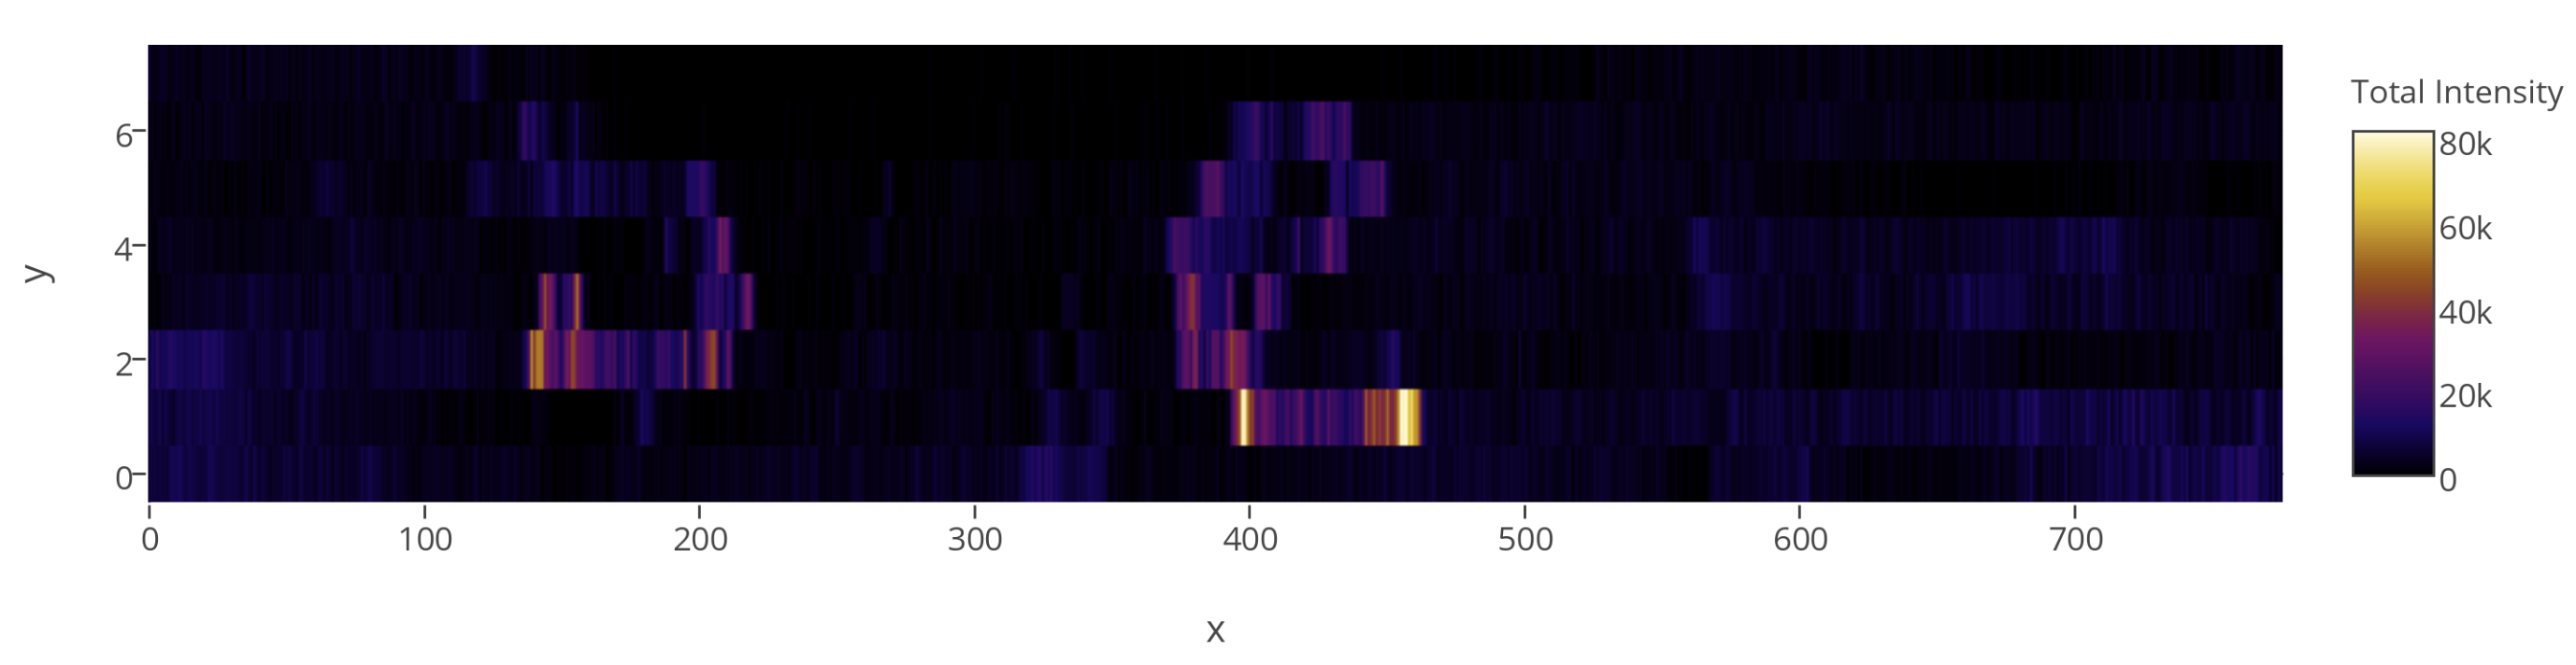
\includegraphics[width=\linewidth]{pre.png}
  \end{subfigure}%

  \begin{subfigure}[b]{0.5\textwidth}
    \caption{The term's occurrences after linear baseline scaling.}
    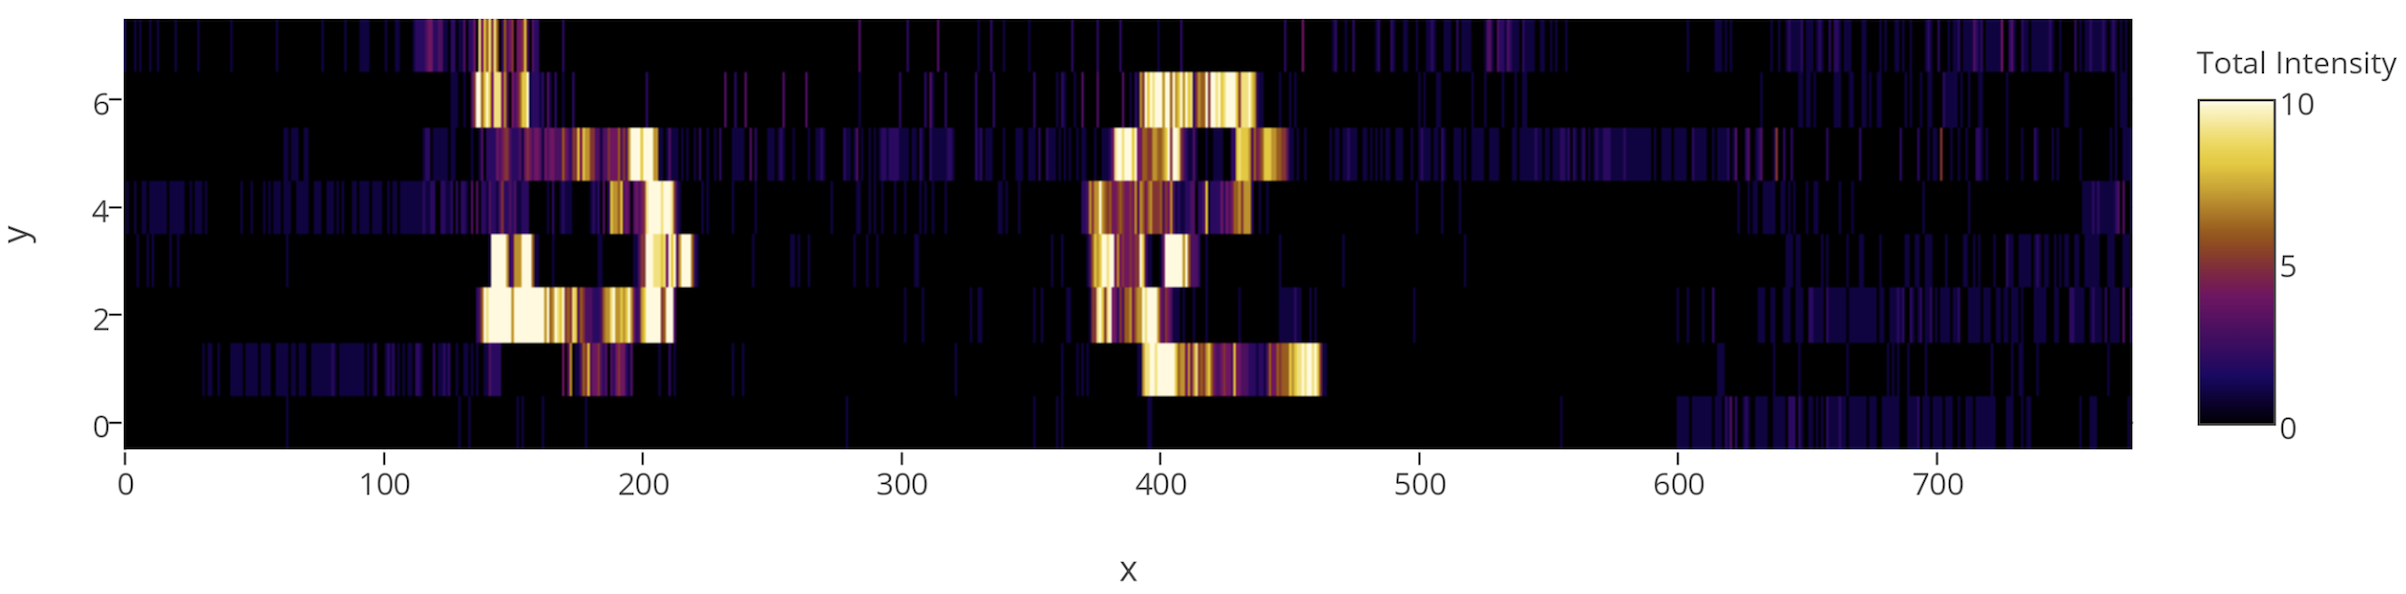
\includegraphics[width=\linewidth]{post.png}
  \end{subfigure}%

  \begin{subfigure}[b]{0.5\textwidth}
    \caption{An inferred topic corresponding to the pattern.}
    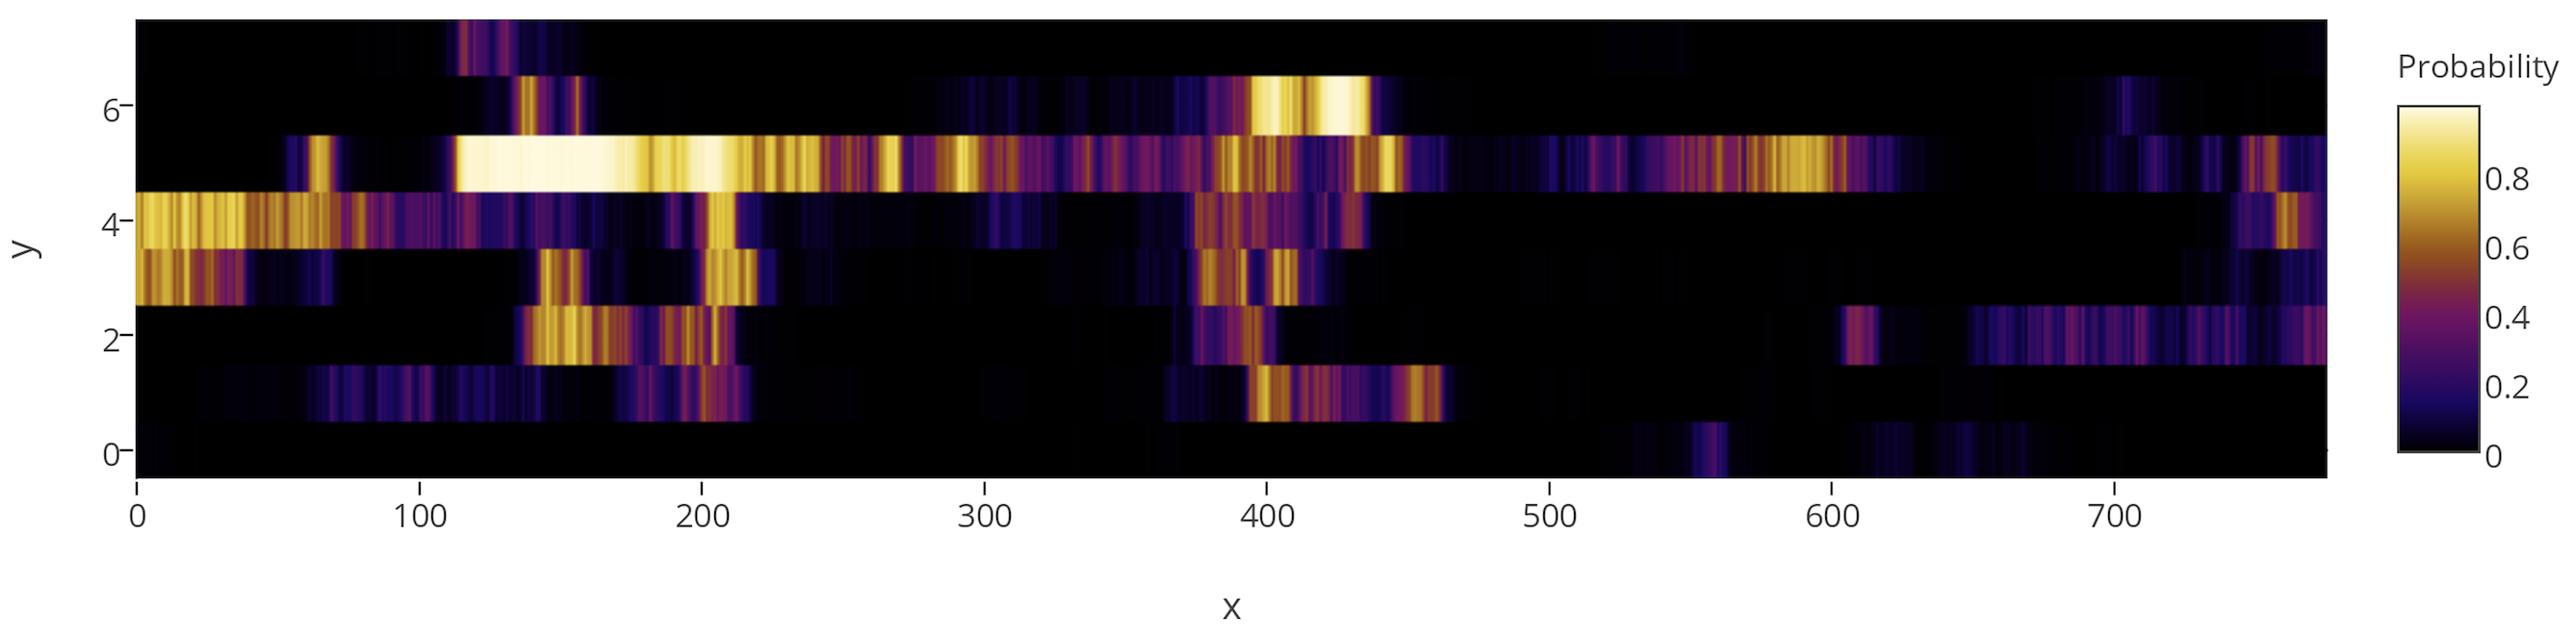
\includegraphics[width=\linewidth]{topic.png}
  \end{subfigure}%
  \caption{The term's visual comparison.}
  \label{fig:comparison}
\end{figure}

% The generative process
% - The underlying assumption for the inference
% - synthetic data
% -- Large amounts of data
% - The algorithm of the generative process
% - 1 document is 1 segment
\par Having a basis for a scalable inference, we transfer the identified data properties into the synthetic corpus generation. Before introducing the generative process, recall that our dynamic topic treatment is unique with respect to every document. Therefore, contrary to the reviewed dynamic topic models, our dynamic segment consists of only one document. Applying the latter aspects, we establish our utilised generative process given in Algorithm \ref{alg:dynamic_document_generation} below:
\begin{algorithm}[H]
\caption{The generative process for a synthetic corpus.}
\label{alg:dynamic_document_generation}
\begin{algorithmic}[2]
% \State $\alpha_0 \sim \mathcal{N}(0, \sigma_0^2I)$
\For {$t \leftarrow 1, T$}
% \State $\alpha_t \sim \mathcal{N}(\alpha_{t-1}, \sigma^2I)$
\State $N \sim \mbox{Poisson}(\xi)$
\For {$n \leftarrow 1, N$}
\State $z_{t, n} \sim \mbox{Multinomial}(\pi(\alpha_t))$
\State $k = \{i : z_{t, n, i} = 1\}$
\State $w_{t, n} \sim \mbox{Multinomial}(\phi_k)$
\EndFor
\EndFor
\end{algorithmic}
\end{algorithm}
In practical settings, the rationale of the generative process is defined as follows: the $\xi$ term represents an approximate number of words per document; $\alpha_t$ is the pre-defined auto-regressive hyper-parameter for document $t$; and $\phi_k$ is the pre-defined vocabulary term distribution for topic $k$.


% ___________________________________________________________________________
 \section{Experiments}

% Introduce Non-AR model
% Experiment: AR tuning

\lipsum[1-3]

% ___________________________________________________________________________
\section{Conclusion}

\lipsum[1]

% ___________________________________________________________________________
\bibliographystyle{abbrv}
\bibliography{bibliography}

\end{document}